\documentclass[preprint,12pt]{elsarticle}
\biboptions{sort&compress}
\usepackage{amsmath}
\usepackage{amsfonts}
\usepackage{amssymb}
\usepackage{graphicx}
\usepackage{hyperref}
\usepackage{tabls}
\usepackage{multirow}
\usepackage{cleveref}
\usepackage{verbatim}

\usepackage{pgfplots}
\usetikzlibrary{plotmarks}
\usepackage{tikz}
\usetikzlibrary{shapes,arrows}
\newcommand*{\h}{\hspace{5pt}}% for indentation
\newcommand*{\hh}{\h\h}% double indentation

\usepackage{framed} % Framing content
\usepackage{multicol} % Multiple columns environment
\usepackage{nomencl} % Nomenclature package
\RequirePackage{ifthen}
\renewcommand{\nomgroup}[1]{%
\ifthenelse{\equal{#1}{P}}{\item[\textbf{Superscripts}]}{
\ifthenelse{\equal{#1}{G}}{\item[\textbf{Greek Symbols}]}{
\ifthenelse{\equal{#1}{S}}{\item[\textbf{Subscripts}]}{}}}}

\newcommand{\nomunit}[1]{%
\renewcommand{\nomentryend}{\hspace*{\fill}#1}}
\newcommand{\bv}[1]{\boldsymbol #1}  % change this to change how math vectors are handled

%\usepackage{breqn}

%\special{papersize=8.5in,11in}

\journal{International Journal of Heat and Mass Transfer}


\pdfinfo{%
  /Title(Optimization of an Inverse Convection Solution Strategy)
  /Author   (Yogesh Jaluria)
    /Author   (Joseph R VanderVeer)
  /Creator  (Joseph R VanderVeer)
  /Subject  (Inverse Convection Problems)
}

\begin{document}

\begin{frontmatter}
\title{Optimization of an Inverse Convection Solution Strategy}

\author{Joseph R VanderVeer}
\author{Yogesh Jaluria\corref{cor}}
\ead{jaluria@soemail.rutgers.edu}

\address{Department of Mechanical and Aerospace Engineering: Rutgers University, 98 Brett Rd, Piscataway NJ, 08854}
\cortext[cor]{Corresponding Author}



\begin{abstract}



\end{abstract}
\begin{keyword}
Inverse Problems \sep Computational Heat Transfer \sep Convection
\end{keyword}
\end{frontmatter}

\crefname{equation}{equation}{equations}
\crefname{figure}{figure}{figures}
\crefname{table}{table}{tables}

\newlength\figureheight 
\newlength\figurewidth 
	
	
	
	
\makenomenclature
\setlength{\nomitemsep}{-\parskip} % Baseline skip between items
\renewcommand*\nompreamble{\begin{multicols}{2}}
\renewcommand*\nompostamble{\end{multicols}}
\nomenclature[A]{$T$}{temperature}
\nomenclature[G]{$\bv{\Delta}$}{relative difference between the first sampled point and other sampled points}
\nomenclature[A]{$\bv{r}$}{vector location of sampled points}
\nomenclature[A]{$F$}{minimization function}
\nomenclature[A]{$n$}{number of sample locations}
\nomenclature[G]{$\bv{\delta}$}{vector distance between the actual sampled location and the current test location}
\nomenclature[G]{$\varepsilon$}{error associated with the inverse convection method at a location with given sampled data}
\nomenclature[A]{$d$}{number of simulations}
\nomenclature[A]{$a$}{number of sample locations used in the predictor stage}
\nomenclature[A]{$U$}{free stream velocity}
\nomenclature[A]{$x,y$}{coordinates}
\nomenclature[G]{$\phi$}{normalized temperature $\phi = \frac{T-T_{\infty}}{T_S-T_{\infty}}$}
\nomenclature[A]{$X,Y$}{normalized coordinates}
\nomenclature[S]{$i, j,k$}{index}
\nomenclature[S]{$A,B$}{data set A,B}
\nomenclature[S]{$P$}{predicted}
\nomenclature[S]{$mod$}{modified}
\nomenclature[S]{$\infty$}{free stream}
\nomenclature[P]{$\ast$}{predictor stage, alternative heat flux eqn.}
\nomenclature[S]{$S$}{source}
\nomenclature[A]{$b,m$}{model parameters}
\nomenclature[S]{$0,1,2$}{sample point indexes}
\nomenclature[S]{$O$}{optimized}
\nomenclature[G]{$\rho$}{density}
\nomenclature[A]{$t$}{time}
\nomenclature[A]{$P$}{pressure}
\nomenclature[A]{$E$}{thermal energy}
\nomenclature[G]{$\mu_{t}$}{eddy viscosity}
\nomenclature[A]{$P_{rt}$}{turbulent Prandtl number}
\nomenclature[A]{$k,\epsilon$}{turbulence kinetic energy, dissipation rate}
\nomenclature[A]{$C_1,C_2,C_{1\epsilon},C_{\mu},\sigma_k,\sigma_{\epsilon}$}{$k-\epsilon$ model coefficients}
\nomenclature[A]{$l, I$}{turbulence length scale and intensity}
\nomenclature[G]{$\lambda$}{thermal conductivity}
\nomenclature[G]{$\mu$}{dynamic viscosity}

%\nomenclature[A]{ }{ }

\begin{table*}[!t]
  \begin{framed}
    \printnomenclature
  \end{framed}
\end{table*}




\section{Introduction}
Thermal-fluid systems often create situations where the engineering problem is an inverse heat transfer problem.  These problems often have limited physical access, very limited to no boundary condition knowledge, and/or limited domain knowledge.

For example, the temperature distribution of an optical fiber drawing furnace is difficult to measure directly due to shape, inaccessibility, and high temperatures.  The center of the furnace is easily accessible and this directly leads to an inverse heat transfer problem.  \Citet{issa} \cite{iss} developed a regularization technique utilizing the centerline temperature from which the wall temperature may be obtained.

Another example, is the inverse plume in a crossflow problem.  The problem entails solving for the plume boundary conditions utilizing limited domain knowledge.  A novel predictor-corrector method was developed by \citet{ijhmt1} \cite{ijhmt1} to solve such a problem.  


The present work is the logical progression of the inverse plume in a crossflow problem, the inverse jet in a crossflow problem.  The inverse jet in a crossflow problem has many more practical applications and ...





\section{Experimental System}
The experiment consists of a wind tunnel with a surface level jet located within the test section.  The jet uses compressed air passed through flow straighteners to achieve a velocity of $U_S$ and is heated to temperature $T_S$.  The jet is subjected to a perpendicular crossflow of velocity $U_{\infty}$.  \Cref{fig:diagramjet} is a diagram of the wind tunnel and jet, dimensions are in millimeters.

\begin{figure}[!tbp]
\begin{center}
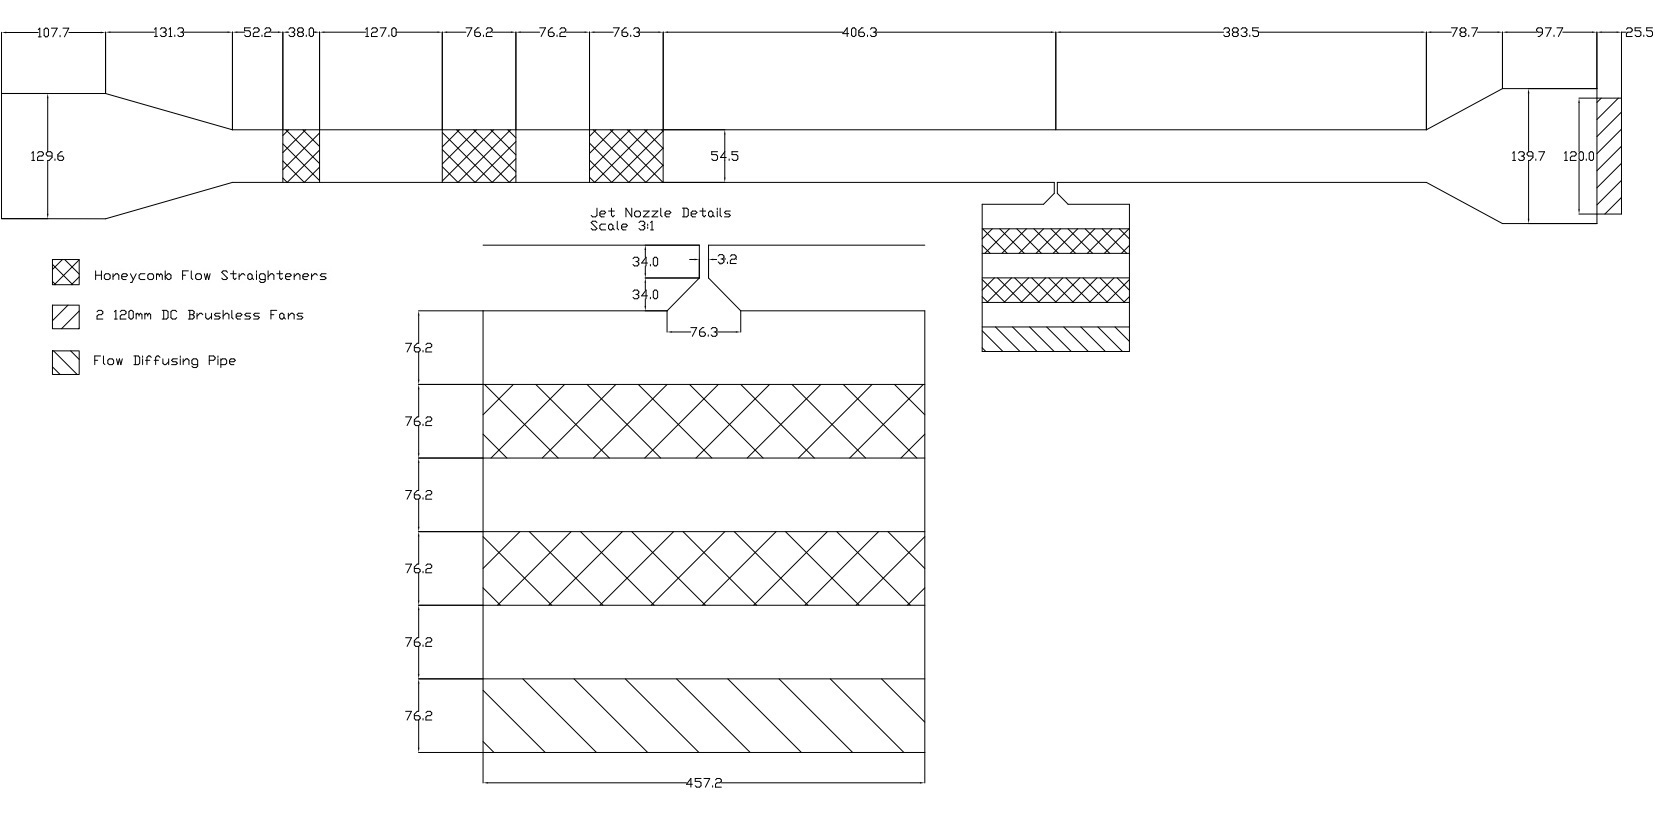
\includegraphics[scale=.30]{windtunneljet.jpg}
\caption{Schematics of the wind tunnel and jet}
\label{fig:diagramjet}
\end{center}
\end{figure}

The wind tunnel test section dimensions are $54.5\times305\times 254\,mm$.  The maximum velocity of the wind tunnel is $5.0\,m/s$.  The jet is heated by electric cartridge heaters with a maximum temperature of $425\,K$ due to material limitations of the wind tunnel.  The X-direction is directed downstream of the wind tunnel with the zero at the center of the jet.  The Y-direction is in the direction of the jet and is zero at the surface of the wind tunnel.  Due to the large aspect ratio of the wind tunnel the flow is assumed to be two-dimensional.

The free stream velocity is determined by a Pitot-Static tube attached to a NIST traceable differential pressure sensor from Omega(PX655-0.1DI).  The pressure sensor has a full scale reading of 0.1 inches of water and is accurate to $0.05\%$ of full scale.  This results in a maximum of $3\%$ error of the calculated velocity.

The jet velocity is determined utilizing a rotameter and verified using a Pitot-Static tube attached to the same previously described pressure sensor.  This results in the same amount of error of $3\%$ for the jet velocity.

The temperature of domain is measured using a K-type thermocouple mounted to an X-Y traversing stage.  Sampled data over the course of several days indicate repeatability of the experiment to within $2\%$.

\section{Numerical Simulations}
The simulations were all performed using Ansys Fluent\cite{fluentsoftware}.



\section{Inverse Solution Methodology}





\section{Results and discussions}


\section{Conclusions}

\appendix

\bibliography{Bibliography}{}
\bibliographystyle{model1-num-names}
\end{document}

